\begin{figure}[tb]
\centering
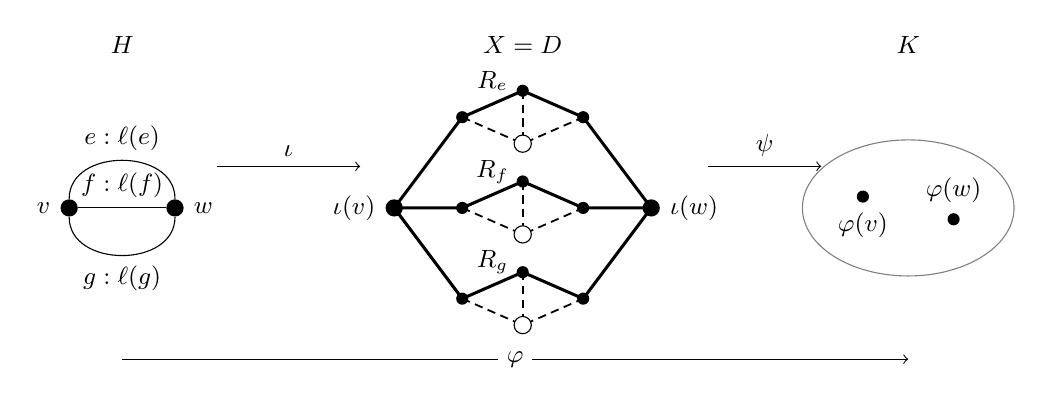
\begin{tikzpicture}[
  x=.96cm,y=.96cm,
  every node/.style={font=\small},
  vertex/.style={circle,fill=black,inner sep=1.55pt},
  branch/.style={circle,fill=black,inner sep=2.2pt},
  outside/.style={circle,draw=black,fill=white,inner sep=2.2pt},
  route/.style={line width=1.1pt},
  perron/.style={densely dashed,line width=.65pt},
]
\node at (0,2.15) {$H$};
\node at (5.3,2.15) {$X=D$};
\node at (10.4,2.15) {$K$};
\node[branch,label=left:$v$] (hu) at (-.7,0) {};
\node[branch,label=right:$w$] (hv) at (.7,0) {};
\draw (hu) .. controls (-.7,.8) and (.7,.8) .. (hv)
  node[midway,above] {$e:\ell(e)$};
\draw (hu)--(hv) node[midway,above] {$f:\ell(f)$};
\draw (hu) .. controls (-.7,-.8) and (.7,-.8) .. (hv)
  node[midway,below] {$g:\ell(g)$};

\coordinate (xu) at (3.6,0);
\coordinate (xv) at (7,0);
\foreach \height/\j in {1.2/e,0/f,-1.2/g} {
  \coordinate (a\j) at (4.5,\height);
  \coordinate (b\j) at (6.1,\height);
  \coordinate (c\j) at (5.3,\height+.35);
  \coordinate (d\j) at (5.3,\height-.35);
  \draw[perron] (a\j)--(d\j)--(b\j);
  \draw[perron] (c\j)--(d\j);
  \draw[route] (xu)--(a\j)--(c\j)--(b\j)--(xv);
  \foreach \p in {a,b,c} {\node[vertex] at (\p\j) {};}
  \node[outside] at (d\j) {};
  \node at (4.9,\height+.48) {$R_\j$};
}
\node[branch,label=left:$\iota(v)$] at (xu) {};
\node[branch,label=right:$\iota(w)$] at (xv) {};

\draw[black!50] (10.4,0) ellipse (1.4 and .9);
\node[vertex,label=below:$\varphi(v)$] at (9.8,.15) {};
\node[vertex,label=above:$\varphi(w)$] at (11,-.15) {};
\draw[->] (1.25,.55)--(3.15,.55) node[midway,above] {$\iota$};
\draw[->] (7.75,.55)--(9.25,.55) node[midway,above] {$\psi$};
\draw[->] (0,-2)--(10.4,-2)
  node[midway,fill=white,inner sep=3pt] {$\varphi$};
\end{tikzpicture}
\caption{The objects in \cref{lem:perron-transfer}, using $D$ from
\cref{fig:diamond-objects}.
Edges of $R_e$ have label $\ell(e)$; each solid path has three internal vertices.
Dashed edges have label $\rho_K$; hollow vertices lie outside all $R_e$.
The target $K$ is schematic, with two vertex images marked.
The coefficient $c_K(X,\ell_X)$ sums over all maps $\psi:V(X)\to V(K)$;
the right side of \cref{eq:perron-transfer} sums over all
$\varphi:V(H)\to V(K)$.
For a fixed $\psi$, we have $\varphi=\psi\circ\iota$.}
\label{fig:perron-objects}
\end{figure}
